\chapterimage{chapter_head_2.pdf} % Chapter heading image

\chapter{Física - 1as séries}

\section{Conceitos iniciais}\index{Conceitos iniciais}
O objetivo deste material é direcionar os conteúdos de Física do Ensino Médio de modo mais sucinto e objetivo com exemplos preparados pelo autor.

A estrutura será mostrada de acordo com os bimestres de cada série baseado nas habilidades essenciais do Currículo Paulista.

Em cada exemplo haverá alguns códigos das habilidades de acordo com o Currículo, pode ser que haja mais de um código, mas serão colocados os principais.

\section{Grandezas}\index{Grandezas}
Na Física, grandezas são as propriedades físicas que podem ser medidas, tais como comprimento, massa, tempo, temperatura, velocidade, aceleração, energia, entre outras. Essas grandezas são quantificadas por meio de unidades de medida, que permitem comparar e relacionar as diferentes grandezas. A utilização das grandezas e unidades é essencial para a realização de experimentos e cálculos na Física, permitindo a descrição e explicação dos fenômenos físicos de forma precisa e objetiva. Além disso, as grandezas físicas estão presentes em diversas áreas do conhecimento, desde a mecânica até a termodinâmica, e são fundamentais para o avanço da ciência e tecnologia.
\subsection{Escalares}\index{Escalares}
As grandezas escalares na Física são aquelas que possuem apenas um valor numérico e uma unidade de medida, sem a necessidade de uma direção específica. Exemplos de grandezas escalares incluem a massa, a temperatura, o tempo, a energia, a pressão, entre outras. A característica fundamental das grandezas escalares é que elas podem ser somadas, subtraídas, multiplicadas e divididas sem a necessidade de uma orientação específica. Além disso, a representação gráfica das grandezas escalares é feita por meio de uma única dimensão, geralmente representada por uma reta numérica. As grandezas escalares são de grande importância na Física, pois permitem a realização de cálculos e análises precisas dos fenômenos físicos, sendo utilizadas em diversas áreas do conhecimento.
\subsection{Vetoriais}\index{Vetoriais}
As grandezas vetoriais na Física são aquelas que possuem tanto um valor numérico quanto uma direção e um sentido específicos. Exemplos de grandezas vetoriais incluem a velocidade, a aceleração, a força, o momento angular, entre outras. A característica fundamental das grandezas vetoriais é que elas não podem ser somadas ou subtraídas diretamente, uma vez que a soma de vetores depende não apenas dos seus valores numéricos, mas também das suas direções e sentidos. A representação gráfica das grandezas vetoriais é feita por meio de vetores, que são segmentos de reta orientados, representando a direção e sentido da grandeza. As grandezas vetoriais são de grande importância na Física, pois permitem a descrição precisa de fenômenos físicos complexos, além de serem fundamentais para o cálculo de grandezas como a resultante de forças e a trajetória de um objeto em movimento.


\section{Soma de vetores}\index{Soma de vetores}






\section{Termologia}\index{Termologia}
\subsection{Escalas temométricas}\index{Escalas termométricas}
As escalas mais conhecidas (Celsius e Fahrenheit) foram construídas usando, basicamente, a transição de estados da água: fusão e ebulição. A escala Kelvin (escala absoluta) também pode ser definida como segue:

\begin{table}[!h]
    \centering
    \caption{Escalas mais conhecidas e seus valores para os pontos de fusão e ebulição da água}
    \vspace{.5cm}
    \label{tab:my-table}
    \begin{tabular}{cccc}
    \textbf{Escala}                    & \textbf{Celsius {[}°C{]}} & \textbf{Fahrenheit {[}°F{]}} & \textbf{Kelvin {[}K{]}} \\
    \textbf{Ponto de ebulição da água} & 100                       & 212                          & 373,15                  \\
    \textbf{Ponto de fusão da água}    & 0                         & 32                           & 273,15                 
    \end{tabular}
\end{table}


\begin{figure}[!h]
    \caption{Representação das escalas termométricas}
    
    \centering % para centralizarmos a figura
    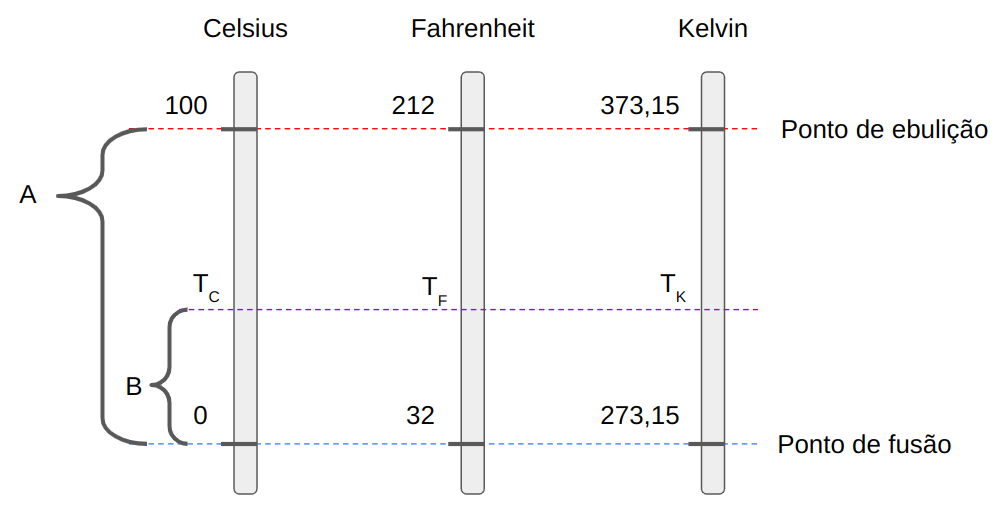
\includegraphics[width=12cm]{Pictures/FISICA_EM/TERMOLOGIA/escalas_termometros.png} % leia abaixo
    \label{figura:qualquernome}
\end{figure}

Como pode ser visto na figura acima, é possível estabelecer relações entre as escalas de modo a converter as temperaturas. Uma forma de estabelecer as conversões entre as escalas é fazer a proporção entre as razões $A/B$ de cada escala, assim:

\begin{ceqn}
\begin{align*}
    \frac{T_C - 0}{100 - 0} = \frac{T_F - 32}{212 - 32} = \frac{T_K-273,15}{373,15 - 273,15}
\end{align*}
\begin{align*}
    \frac{T_C}{100} = \frac{T_F - 32}{180} = \frac{T_K-273,15}{100}
\end{align*}
\end{ceqn}

Através da relação acima, é possível relacionar as escalas e fazer a conversão entre elas, como segue:

\subsubsection{Relação entre Celsius e Fahrenheit}
\begin{ceqn}
    \begin{align*}
        \frac{T_C}{100} &= \frac{T_F - 32}{180} \\
        \frac{180 \cdot T_C}{100} &= T_F -32 \\
        \frac{9}{5} \cdot T_C &= T_F-32 \\
    \end{align*}
\end{ceqn}

\subsubsection{Relação entre Celsius e Kelvin}
\begin{ceqn}
    \begin{align*}
        \frac{T_C}{100} &= \frac{T_K-273,15}{100} \\
        T_C&=T_K-273,15 \\
    \end{align*}
\end{ceqn}

\subsubsection{Relação entre Fahrenheit e Kelvin}
\begin{ceqn}
    \begin{align*}
        \frac{T_F - 32}{180} &= \frac{T_K-273,15}{100} \\
        \frac{100}{180}\cdot (T_F-32) &= T_K-273,15 \\
        \frac{5}{9} \cdot (T_F-32) &= T_K-273,15 \\
    \end{align*}
\end{ceqn}



\begin{example}
Calcule a temperatura em graus Fahrenheit sabendo que a temperatura em ${}^\text{o}$C é de 32.

\begin{ceqn}
\begin{align*}
\frac{9}{5} \cdot T_C =& T_F - 32 \\
\frac{9}{5} \cdot 32 =& T_F - 32 \\
1,8 \cdot 32 =& T_F - 32 \\
57,6 =& T_F -32 \\
T_F =& 57,6 + 32 \\
T_F =& 89,6 {}^oF \\
\end{align*}
\end{ceqn}
\end{example}
